% mnras_template.tex
%
% LaTeX template for creating an MNRAS paper
%
% v3.0 released 14 May 2015
% (version numbers match those of mnras.cls)
%
% Copyright (C) Royal Astronomical Society 2015
% Authors:
% Keith T. Smith (Royal Astronomical Society)

% Change log
%
% v3.0 May 2015
%    Renamed to match the new package name
%    Version number matches mnras.cls
%    A few minor tweaks to wording
% v1.0 September 2013
%    Beta testing only - never publicly released
%    First version: a simple (ish) template for creating an MNRAS paper

%%%%%%%%%%%%%%%%%%%%%%%%%%%%%%%%%%%%%%%%%%%%%%%%%%
% Basic setup. Most papers should leave these options alone.
\documentclass[a4paper,fleqn,usenatbib]{mnras}

% MNRAS is set in Times font. If you don't have this installed (most LaTeX
% installations will be fine) or prefer the old Computer Modern fonts, comment
% out the following line
\usepackage{newtxtext,newtxmath}
% Depending on your LaTeX fonts installation, you might get better results with one of these:
%\usepackage{mathptmx}
%\usepackage{txfonts}

% Use vector fonts, so it zooms properly in on-screen viewing software
% Don't change these lines unless you know what you are doing
\usepackage[T1]{fontenc}
\usepackage{ae,aecompl}


%%%%% AUTHORS - PLACE YOUR OWN PACKAGES HERE %%%%%

% Only include extra packages if you really need them. Common packages are:
\usepackage{graphicx}	% Including figure files
\usepackage{amsmath}	% Advanced maths commands
\usepackage{amssymb}	% Extra maths symbols

\usepackage[flushleft, referable]{threeparttablex} % Adding notes under tables
\usepackage{mhchem} 	% typeset chemistry symbols
\usepackage{multicol} 	% Multi-column entries in tables
% \usepackage{natbib} % references in text to look like MNRAS/ApJ/A&A
% \usepackage{multirow} % for multirow command
% \usepackage{array} % For wrapping text in cell in tables




%%%%%%%%%%%%%%%%%%%%%%%%%%%%%%%%%%%%%%%%%%%%%%%%%%

%%%%% AUTHORS - PLACE YOUR OWN COMMANDS HERE %%%%%

% Please keep new commands to a minimum, and use \newcommand not \def to avoid
% overwriting existing commands. Example:
%\newcommand{\pcm}{\,cm$^{-2}$}	% per cm-squared
\defcitealias{Thomas2010}{TMJ} % TMJ alias
% \newcolumntype{L}[1]{>{\raggedright\let\newline\\\arraybackslash\hspace{0pt}}m{#1}} % 
\newcommand{\bracket}[1]{[#1]} % to be able to use [] in arguments


%%%%%%%%%%%%%%%%%%%%%%%%%%%%%%%%%%%%%%%%%%%%%%%%%%

%%%%%%%%%%%%%%%%%%% TITLE PAGE %%%%%%%%%%%%%%%%%%%

% Title of the paper, and the short title which is used in the headers.
% Keep the title short and informative.
\title[An IFS study of Low-powered Radio Galaxies]{An IFS study of Low-powered Radio Galaxies}

% The list of authors, and the short list which is used in the headers.
% If you need two or more lines of authors, add an extra line using \newauthor
\author[J. Warren et al.]{
Joshua Warren,$^{1}$\thanks{Contact e-mail: \href{mailto:joshua.warren@physics.ox.ac.uk}{joshua.warren@physics.ox.ac.uk}}
Martin Bureau,$^{1}$
Bernd Hasemann,$^{2}$
Isabella Prandoni,$^{3}$ \newauthor
Francesco Santoro,$^{3}$
Robert Laing,$^{3}$
Paola Parma,$^{3}$
Hans de Ruiter$^{3}$
and \newauthor
Arturo Mignano$^{3}$
\\
$^{1}$Sub-department of Astrophysics, Department of Physics, University of Oxford, Denys Wilkinson Building, Keble Road, Oxford OX1 3RH, UK\\
$^{2}$European Southern Observatory, Karl-Schwarzschild-Str. 2, 85748 Garching b. München, Germany\\
$^{3}$INAF - Istituto di Radioastronomia, Via P. Gobetti 101, 40129 Bologna, Italy}


% These dates will be filled out by the publisher
\date{Accepted XXX. Received YYY; in original form ZZZ}

% Enter the current year, for the copyright statements etc.
\pubyear{2018}

% Don't change these lines
\begin{document}
\label{firstpage}
\pagerange{\pageref{firstpage}--\pageref{lastpage}}
\maketitle

% Abstract of the paper
\begin{abstract}
This is a simple template for authors to write new MNRAS papers.
The abstract should briefly describe the aims, methods, and main results of the paper.
It should be a single paragraph not more than 250 words (200 words for Letters).
No references should appear in the abstract.
\end{abstract}

% Select between one and six entries from the list of approved keywords.
% Don't make up new ones.
\begin{keywords}
% keyword1 -- keyword2 -- keyword3
\end{keywords}

%%%%%%%%%%%%%%%%%%%%%%%%%%%%%%%%%%%%%%%%%%%%%%%%%%

%%%%%%%%%%%%%%%%% BODY OF PAPER %%%%%%%%%%%%%%%%%%


\section{Introduction}
	\label{sec:intro}
	% There are known to be strong scaling relations between the mass of the central supermassive black-hole (SMBH) and the global properties in a given galaxy, such as velocity dispersion, the $M-\sigma$ relation \citep{Ferrarese2000, Gebhardt2000, Graham2011}; Sersic index \citep{Graham2007, Savorgnan2013}; luminosity \citep{Laor2001, McLure2001, Lauer2007, Graham2012}; etc. AGN feedback is understood to be the mechanism by which the SMBH can expand its sphere of influence to galactic scales to affect these relationship. 

	% This is generally understood to be a feedback process, where large amounts of gas within the galaxy cools, falls on the SMBH. Here the black-hole imparts energy to the gas, causing outflows (or jets) and/or thermal emission. We observe this as an Active Galactic Nuclei (AGN) which can have distinctive emission across the electromagnetic spectrum. The exact mechanisms of imparting energy still remains an open question, with much theoretical and observational work ongoing. The outflows can then effect the outer parts of the galaxy, by methods such as fountain effects \citep{}, thermal heating \citep{DeYoung2010} and shocks created by the outflows \citep{}.

	% One identifier of AGNs is a radio signature consistent with Synchrotron emission from the outflow i.e a radio galaxy (RG). These are typically categorized into one of two classes: Fanaroff-Riley (FR) I or FR II \citep{Fanaroff1974}. Of these we focus on the former since these are by far the most common mode in the local universe (possibly as far as $z \sim 1$ \citep{Rigby2008}), and so to discuss radio AGN feedback is to consider feedback from FR I sources \citep{DeYoung2010}. Indeed, while there is broad consensus \citep{Heckman1986, Baum1992} that the brightest RGs (mostly FR IIs) are caused when a massive galaxy merges with a gas rich galaxy (a wet merger) giving a plentiful fuel reservoir to the AGN \citep{Baum1992}, there is much more debate when it comes to low-powered ($P_\text{1.4 GHz} \lesssim 10^{24.5} \, \mathrm{W Hz^{-1}}$) RGs (mostly FR I). Suggestions fall into two categories: an extrapolation of radio-loud galaxies (i.e. a merger with either small gas reservoirs or low efficiency accretion onto the SMBH) or a highly efficient accretion of gas from secular origins (such as Bondi accretion of the hot X-ray component of the Inter-Stellar Medium (ISM) \citep{Allen2006} or from existing cold gas reservoirs \citep{Prandoni2010}). This project aims to add to this discussion using Integral Field Unit (IFU) observations in the visible band of nearby radio galaxies and comparing this with Atlas-3D sample \citep{Cappellari2011} as a control sample.

% More to add to intro - e.g. summery of paper 

	We refer to the combined Atlas$^\text{3D}$ and MASSIVE sample as the A+M sample.

\section{Sample Description}
	\label{sec:samp}
	The Parkes 2.7 GHz survey \citep{Ekers1989} was used as a parent sample, as it contains radio sources (down to a flux density limit of 250\,mJy at 2.7\,GHz) with an optical counterpart (with an $V$-band apparent magnitude of $m_V \le 17.0$). Host galaxies with a redshift greater than 0.03 were discarded. It is worth noting that both the radio and optical limits are apparent measurements, and as such this is not a volume-limited sample.

	\begin{table*}
		% \centering
	% \begin{threeparttable}
		\caption{Key sample characteristics of the Southern Sample galaxies. Col.\,1: host galaxy name. Col.\,2: radio source name from Parkes Southern Radio Source Catalogue. We hereafter refer to the last galaxy by its PKS name only. Col.\,3: redshift. Col.\,4: National Radio Astronomy Observatory (NRAO) Very Large Array (VLA) Sky Survey (NVSS) 1.4 GHz flux density \citep{Condon1998}. Col.\,5: Two Micron All Sky Survey (2MASS) $K$-band apparent magnitude (with errors of $\pm 0.025$ mag; \citealt{Skrutskie2006}). Col.\,6: dust morphologies from (a) \citet{Govoni2000}, (b) \citet{Lauer2005}, (c) \citet{Bettoni2001}, (d) \citet{Sandage1979}, (e) \citet{Colbert2001}.}
		\label{tab:sample}
		\begin{tabular}{l c c c c l}
			\hline
			\hline
			Host galaxy	& Radio source 	& Redshift	& $S_\text{1.4\,GHz}$	& $m_K$ & Dust morphology\\
						& (PKS) 		& 			& (mJy) 			& (mag)	&\\
			\hline 
			ESO 443-G024 & 1258-321 	& 0.01703	& $1387 \pm 45$		& 8.51 & no dust\tnote{a}	\\ 
			IC 1459 	& 2254-367 		& 0.00565 	& $1280 \pm 45$		& 6.81 & dust lane\tnote{b}	\\
			IC 1531 	& 0007-325 		& 0.02553 	& \leavevmode\phantom{0}$388 \pm 12$		& 9.55 & --					\\
			IC 4296		& 1333-\leavevmode\phantom{0}33 		& 0.01248 	& $1342 \pm 41$		& 7.50 & edge-on disc\tnote{b} \\
			NGC 612 	& 0131-\leavevmode\phantom{0}36 		& 0.02954 	& \leavevmode\phantom{0}$585 \pm 18$		& 9.58 & dust lane\tnote{c}	\\
			NGC 1316 	& 0320-\leavevmode\phantom{0}37 & 0.00591 	& \leavevmode\phantom{0}$255 \pm 10$		& 5.59 & dust patches\tnote{b} \\
			NGC 1399 	& 0336-\leavevmode\phantom{0}35 & 0.00472 	& \leavevmode\phantom{0}$209 \pm \leavevmode\phantom{0}7$	& 6.31 & no dust\tnote{b}	\\
			NGC 3100 	& 0958-314 		& 0.00879 	& \leavevmode\phantom{0}$530 \pm 16$		& 8.08 & dust lane\tnote{d}	\\
			NGC 3557 	& 1107-372 		& 0.01016 	& \leavevmode\phantom{0}$484 \pm 16$		& 7.20 & face-on disc\tnote{b}\\
			NGC 7075 	& 2128-388 		& 0.01819 	& \leavevmode\phantom{0}$837 \pm 28$		& 9.56 & --					\\
			--			& 0718-\leavevmode\phantom{0}34 		& 0.02897 	& $1119 \pm 41$		& 9.97 & dust patches\tnote{e} \\
			\hline
			\hline
		\end{tabular}
	% 	\begin{tablenotes}
	% 	\footnotesize
	% 	\note Col.\,1: host galaxy name. Col.\,2: radio source name from Parkes Southern Radio Source Catalogue. Col.\,3: redshift. Col.\,4: National Radio Astronomy Observatory (NRAO) Very Large Array (VLA) Sky Survey (NVSS) 1.4 GHz flux density \citep{Condon1998}. Col.\,5: Two Micron All Sky Survey (2MASS) $K$-band apparent magnitude (with errors of $\pm 0.025$ mag; \citealt{Skrutskie2006}). Col.\,6: dust morphologies from (a) \citet{Govoni2000}, (b) \citet{Lauer2005}, (c) \citet{Bettoni2001}, (d) \citet{Sandage1979}, (e) \citet{Colbert2001}. 
	% 	\item We hereafter refer to the last galaxy by its PKS name only.
	% 	\end{tablenotes}
	% \end{threeparttable}
	\end{table*}

	These criteria lead to a sample of 11 galaxies hereafter referred to as the Southern Sample. The key observed characteristics are summarised in Table \ref{tab:sample}.
	%, while the derived characteristics are listed in Table \ref{tab:sampleDerived}. 
	All galaxies have a FR I radio morphology according to the \citet{Fanaroff1974} scheme; the bulk of the radio emission is centrally-concentrated, as opposed to the FR II morphology where the brightest points are at the ends of the radio lobes. 
	
	The sample was initially observed with the Atacama Pathfinder Experiment \citep[APEX; ][]{Gusten2006}, with detections claimed for the \ce{^{12}CO(2-1)} transition for all galaxies. Some galaxies had extremely large line widths (up to a full-width half-maximum of $904 \, \mathrm{km \, s^{-1}}$ for IC 4296), but most showed a flat or double-horn spectrum indicative of ordered rotation \citep{Prandoni2012}.


\section{Observing strategy and Data Reduction}
	\label{sec:obs}
	The sample was observed with the Visible Multi-Object Spectrograph (VIMOS), mounted on UT3 on the VLT in Paranal \citep{LeFevre2003}. All observations were taken with a spatial sampling of $0\farcs67$, using the high-resolution blue grism yielding a wavelength range of 3700-5520\,\AA\ with a spectral resolution of 1440 and sampling of 0.71\,\AA\,$\mathrm{pix^{-1}}$. Each object was observed with a total integration time of $\approx 100$\,min on-source, equally spread over three observing blocks (OBs). Each OB also contained all the necessary observation for standard IFS data reduction. 

	VIMOS has several well-known though poorly-understood technical issues. These include several low transmission (bad) fibres, strong flexure, contamination from adjacent spectra on the CCD (cross-talk) and large differences in sensitivity across its 4 quadrants. To address these issues, we adopted a data-reduction pipeline produced using \textsc{Py3D}, a suite of programs based on the \textsc{python} versions of those developed for the Calar Alto Legacy Integral Field spectroscopy Area survey \citep[CALIFA;][]{Sanchez2012, Husemann2013} but later updated for VIMOS by \citet{Husemann2014}. \textsc{Py3D} applies all standard IFS data-reductions steps: bias subtraction, spectrum identification, flatfielding and wavelength calibration. In addition, the data was flux calibrated using publicly available observations of the spectro-photometric standard star Feige 110 provided by ESO. All steps include methods to account for the bad fibres, flexure and cross-talk within VIMOS. 

	Following this, we noted that the cubes where still not properly calibrated. Three main issues remain: the quadrants have different intensities, clearly showing uncorrected throughput differences; diagonal intensity stripes are present in the reconstructed images at all wavelengths; and spectral features are observed \citep{Jullo2008} that are visually similar to fringe patterns caused by interference within the CCD between incident light and light reflected from the interfaces between layers of the CCD materials. \citet{Lagerholm2012} present ad-hoc methods to correct for these issues, which we here adopt. These additional steps mean that the datacubes are not perfectly flux-calibrated, but all the corrections are multiplicative and thus will not effect equivalent width or line ratio measurements. From comparisons to the MUSE data (see Section \ref{subsec:MUSE}), we then estimate the flux calibration of the resulting datacubes. 

	These method are not completely effective and some artefacts are still present in the data, however in most cases the data is of sufficient quality for our purposes. For the worst effected datacubes, we have archival observations (see Section \ref{subsec:MUSE}).

	The variance spectra are propagated throughout the data-reduction pipeline (including these ad-hoc corrections) and are square-rooted at this point, to be used as noise inputs in the following analyses (see Section \ref{sec:analysis}).


	\subsection{MUSE Archival Data}
		\label{subsec:MUSE}
		Four of the sample galaxies are in the Multi-unit Spectroscopic Explorer (MUSE) archive: IC 1459, IC 4296, NGC 1316 and NGC 1399. We include these in our analysis as they have better (spatial and spectral) resolution and sampling, a larger field-of-view and larger wavelength range than the VIMOS data. 

		We used the pre-reduced (Phase 3) datacubes from ESO. These were generally of sufficient quality for our purpose, except in both IC 1459 and IC 4296 the sky appears to have been over-subtracted. To remove this over-subtraction, we developed our own pseudo-sky subtraction routine. A median spectrum was taken from four $20 \times 20$\,spaxel regions, one in from each spatial corner of the ESO reduced cube. After checking that no stellar continuum could be fit to the medium sky spectrum (i.e.\ that very little light from the galaxy is contaminating the pseudo-sky regions), this median sky spectrum was subtracted from each spaxel in the cube. 

		Finally, we trimmed all the MUSE cubes to the central $30\arcsec \times 30\arcsec$ ($150 \times 150$\,spaxels) only, to (a) avoid the regions used for the pseudo-sky spectrum and (b) reduce the computing resources required for spatial binning (see Section \ref{sec:analysis}). In any case, the bins would likely be so large in the outer parts as to be effectively useless.

\section{Data Analysis}
	\label{sec:analysis}
	From this point on, the VIMOS and MUSE datasets are treated almost identically, the only difference (other than the different spectral ranges and resolutions) being that the MUSE datacubes are spatially binned to a higher signal-to-noise ratio (S/N) using Voronoi binning\footnote{http://www-astro.physics.ox.ac.uk/~mxc/software/} \citep{Cappellari2003}. For our purposes, we define the `signal' and `noise' of each spaxel as the median value of its spectrum and noise spectrum, respectively. We require a S/N of 30 for all VIMOS datacubes and 50 for the IC 1459 and IC 4296 MUSE datacubes. The NGC 1316 and NGC 1399 MUSE datacubes were binned to a S/N of 50 for the analysis of the stellar kinematics and 100 for the analysis of the emission line kinematics and stellar populations.

	Next we implement a routine to find optimal initial guesses of the redshift and velocity dispersion for each galaxy, to be used when fitting individual bins, by means of iterative fits to the spatially collapsed (i.e. summed across both spatial dimensions of the datacube) spectrum. We use the penalized-fitting (\textsc{pPXF}) routine\footnote{http://www-astro.physics.ox.ac.uk/~mxc/software/} of \citet{Cappellari2004} and \citet{Cappellari2016a} with the Medium-resolution Issac Newton Telescope (INT) Library of Empirical Spectra (MILES) library \citep{Sanchez-Blazquez2006, Falcon-Barroso2011a} to find the best-fitting line-of-sight velocity distribution (LOSVD; as parametrised by the Gaussian parameters $v$, the mean velocity and $\sigma$, the velocity dispersion). The final mean velocity of a given galaxy, is used as its precise spectroscopic redshift and is given in Table \ref{tab:sample}. Beyond this point, each bin is analysed independently.

	\subsection{Stellar Kinematics}
		\label{subsec:starKin}
		Each bin is fit independently again using \textsc{pPXF} with the MILES library. For the fit regions around potential emission lines are masked, and a fourth order polynomial additive continuum correction is used. A Monte--Carlo (MC) estimate of the uncertainties is used. 

	\subsection{Ionized Gas Distribution and Kinematics}
		\label{subsec:EmissionLines}
		We fit the ionized gas fluxes and kinematics from the emission lines listed in Table \ref{tab:EmissionLine}, using Gaussian templates are used to independently fit emission lines from the interstellar medium (ISM), with a single LOSVDs, independently of the stellar kinematics. However, to minimize template mismatch, whereby emission lines are erroneously fitted to the edges of badly modeled and thus subtracted absorption features, we follow the method set out in \citet{Sarzi2005}, whereby the stellar component is first fitted as above with masked potential emission line regions, followed by the unmasking and fitting of the [\ion{O}{iii}] doublet which sets the kinematics for all the emission lines and finally the amplitude of the remaining emission lines. Some of the forbidden emission lines have the ratio of their amplitudes fixed (see Table \ref{tab:EmissionLine}, Col.\,4).

		\begin{table}
	 		% \centering
	 	% \begin{threeparttable}
	 		\caption{Emission lines considered in the \textsc{pPXF} fits. Col\,1: Emission line name. Col\,2: Emission line rest-frame wavelength. Col\,3: Doublet rest-frame wavelength for forbidden lines. Col\,4: The fixed ratio of the amplitudes of the lines within a doublet. `Free' indicates the amplitudes of both doublet constituents are fit independently of each other.}
	 		\label{tab:EmissionLine}
	 		\begin{tabular}{l c c c}
	 		\hline
	 		\hline
	 		Emission & Rest-frame & Doublet rest-frame & Amplitude  \\
	 		Line & wavelength & wavelength & ratio \\
	 		 & (\AA) & (\AA) \\
	 		\hline
	 		\bracket{\ion{O}{ii}} 	& 3726.03 & 3728.82 & Free \\
	 		H\,$\delta$ 	& 4101.76 & -- & -- \\
	 		H\,$\gamma$ 	& 4340.47 & -- & -- \\
	 		H\,$\beta$ 		& 4861.33 & -- & -- \\
	 		\bracket{\ion{O}{iii}}	& 4958.92 & 5006.84 & 0.35 \\
	 		\bracket{\ion{N}{i}} 	& 5199.36 & 5201.86 & 0.65 \\
	 		\bracket{\ion{O}{i}} 	& 6300.30 & 6363.67 & 0.33 \\
	 		\bracket{\ion{N}{ii}} 	& 6548.03 & 6583.41 & 0.34 \\
	 		H\,$\alpha$ 	& 6562.30 & -- & -- \\
	 		\bracket{\ion{S}{ii}} 	& 6716.47 & 6730.85 & Free \\
	 		\hline
	 		\hline
	 		\end{tabular}
	 	% 	\begin{tablenotes}
	 	% 	\note Col\,1: Emission line name. Col\,2: Emission line rest-frame wavelength. Col\,3: Doublet rest-frame wavelength for forbidden lines. Col\,4: The fixed ratio of the amplitudes of the lines within a doublet. `Free' indicates the amplitudes of both doublet constituents are fit independently of each other. 
	 	% 	\end{tablenotes}
	 	% \end{threeparttable}
	 	\end{table}


		

	\subsection{Absorption Line Strengths and Stellar Populations}
		\label{subsec:absorption}
		Due to the lack of calibration observations of Lick/Cassegrain Image Dissector Scanner spectrograph system (hereafter Lick/IDS system; \citealt{Faber1985, Worthey1994}) we use the line index system (LIS) of \citet{Vazdekis2010} instead. This relies on flux calibrations instead of correcting to the continuum shape and wavelength dependent resolution of the Lick/IDS system. We use the index definitions of \citet{Trager1998}, measuring the following indices: G4300, Fe4383, Ca4455, Fe4531, H\,$\beta$, Fe5015, Mg\,b, Fe5270, Fe5335, Fe5406, Fe5709, Fe5782, NaD, TiO1 and TiO2. TiO1 and TiO2 are considered molecular absorption lines and are measured in magnitude units, while all others are atomic and measured in angstroms. 

		Quoted line strengths are corrected for both emission line and the effect of the velocity dispersion of the stars. These corrections are detailed below.

		\subsubsection{Removing Emission Lines}
			Emission lines are removed from the spectra by subtracting the best-fitting emission lines from Section \ref{subsec:EmissionLines} from the data and using only the stellar templates (and continuum correction) for reconstructing the best-fit for use in the velocity dispersion correction (see below).

		\subsubsection{Correcting for Stellar Velocity Dispersion}
			We correct for the effect of the different velocity dispersions of the stars which varyingly spread absorption features such that differing fractions of the absorption is outside of the central bandpasses. To do this, we create a best-fitting spectrum (as in the previous step) which is \textit{not} convolved with the best-fitting LOSVD. A given index, $I$, is then measured for both this `unconvolved' spectrum ($I^\text{unc}$) and the convolved best-fitting spectrum ($I^\text{conv}$), and the ratio of these two indices is used as a multiplicative correction factor for the index measured ($I^\text{obs}$), such that the corrected index ($I^\text{corr}$) is given by
			\begin{equation}
				I^\text{corr} \equiv \frac{I^\text{unc}}{I^\text{conv}} I^\text{obs} \, .
			\end{equation}
			These corrected indices are those reported and discussed in the sections below.

		\subsubsection{Best-fitting Stellar Populations}
			\label{subsubsec:stellarPop}
			In each bin, using the measured absorption line strengths, we identify the best-fitting single stellar population (SSP) model from the models of \citeauthor{Thomas2010} (\citeyear{Thomas2010}; hereafter \citetalias{Thomas2010}) using \textsc{emcee}, a \textsc{python}, affine-invariant Markov chain Monte--Carlo (MCMC) fitting package \citep{Foreman-Mackey2013}. The \citetalias{Thomas2010} models are chosen because they are based on high-resolution, flux-calibrated spectra and therefore not requiring absorption line strength measurement to be in the Lick/IDS system.

	\subsection{Other Parameters}
		\subsubsection{Ellipticity}
			In this paper, ellipticity is that of the best-fitting ellipse to the surface-brightness map with an mean radius $R_\text{m}$, of 1 effective radius $R_\text{e}$. % Firstly the centre of the galaxy is found as the luminosity weighted centre using the \textsc{python} routine \textsc{find\_galaxy}, which is part of the \textsc{mge} package\footnote{http://www-astro.physics.ox.ac.uk/\~mxc/software/} by \citet{Cappellari2002}. 
			as found by the \textsc{idl} routine \textsc{kinemetry}\footnote{http://davor.krajnovic.org/idl/} by \citet{Krajnovic2006} which finds the best-fitting ellipses at a range of evenly spaced semi-major axes. %This is achieved by performing harmonic expansion of maps along ellipses with a given semi-major axis and, when used for even moments (e.g.\ surface brightness, velocity dispersion, h$_4$ etc.), minimizing the amplitude of the first and second harmonics. 
			The results include the ellipticity, $\epsilon$ and position angle $PA_\text{phot}$ of the best-fitting ellipse for each semi-major axis. The fit is repeated for increasing semi-major axis until $<$75\% of the ellipse is not contained within the field of view.

			In reality, the field of view does not always contain 1 $R_\text{e}$. Where this is the case, we follow the method by \citet{Emsellem2007}, where $R_\text{m}$ is redefined as $R_\text{m} \equiv \sqrt{A_\text{s}/\pi}$, where $A_\text{s}$ is the area of the ellipse contained within the field of view. For a given galaxy, we fit ellipses as described above, up to $R_\text{m} = R_\text{max}$, where $A_\text{s}$ reaches a maximum difference if 15\% to the area of the fitted ellipse, $A_\text{ellipse}$. The value $\epsilon_\text{e}$, the ellipticity at 1 $R_\text{e}$ or $R_\text{max}$, whichever is smallest, is given in Col.\,3 of Table \ref{tab:classify}. 

		\subsubsection{Kinematic Position Angle}
			The kinematic position angle, $PA_\text{kin}$, is defined as the angle of the axis perpendicular to the apparent angular momentum vector westwards from North. A global value of $PA_\text{kin}$ is found using the \textsc{python} routine \textsc{fit\_kinematic\_pa}\footnote{http://www-astro.physics.ox.ac.uk/\~mxc/software/\#pa\_kin} which finds $PA_\text{kin}$ of the symmetrised mean velocity map, as described in appendix C of \citet{Krajnovic2006}. %This routine finds a symmetric (about $PA_\text{kin}$) velocity field, by replacing the mean velocity, $V$, in each bin with
			% \begin{equation}
			% 	V'(x, y) = \frac{V(x,y) + V(x, -y) - V(-x,y) - V(-x,-y))}{4} \,,
			% \end{equation}
			% where $x$ and $y$ are the centroid coordinates of a given bin, with the origin at the centre of the galaxy and the x axis aligned along $PA_\text{kin}$. Linear interpolation is used where necessary.

			Col.\,4 in Table \ref{tab:classify} lists the misalignments between the photometric and kinematic position angles, $\Gamma_\text{kin} \equiv \arcsin(\sin[PA_\text{phot} - PA_\text{kin}])$.

		\subsubsection{Specific Angular Momentum Parameter, $\lambda_\mathrm{R_e}$}
			We also make use of the Atlas$^\text{3D}$ specific angular momentum parameter, $\lambda_\text{R}$ \citep{Emsellem2007} evaluated at 1 $R_\text{e}$, where 
			\begin{equation}
				\lambda_\mathrm{R_e} \equiv \frac{\sum_{i=1}^{N} F_i R_i |V_i|}{\sum_{i=1}^{N} F_i R_i \sqrt{V_i^2 + \sigma_i^2}}
			\end{equation}
			where $F_i$ is the flux of the $i^\text{th}$ bin, $R_i$ its distance from the centre and $V_i$ and $\sigma_i$ its mean stellar velocity and velocity dispersion, respectively. The sum is computed over all $N$ bins with a radius $R_\text{e}$.

\section{Stellar Kinematics}
	\label{sec:StarKine}
	Using the methods above, we produce stellar kinematic maps for all datacubes (shown in Section \ref{sec:Maps}). Here we use these maps to classify each galaxy according to the Atlas$^\text{3D}$ regular/non-regular rotator and fast/slow rotator classification schemes of \citet{Krajnovic2006} and \citet{Cappellari2016}, respectively, as well as the qualitative kinematic classes of \citet{Krajnovic2011}. We use the criteria described in the referenced literature for each of these classification, with the results shown in Table \ref{tab:classify}.

	\begin{table*}
		% \centering
	% \begin{threeparttable}
		\caption{Kinematic classifications. Col.\,1: Galaxy name. Col.\,2: $\lambda_\text{R}$ evaluated at $R_\text{e}$. Col.\,3: Ellipticity at $R_\text{e}$. Col.\,4: Misalignment angle between the kinematic and photometric position angles. Col.\,5: Fast-/slow-rotator (FR/SR) classification. Col.\,6: Regular-rotator (RR) or non-regular-rotator (NRR). Col.\,7: Kinematic features. Col.\,8: Kinematic group.}
		\label{tab:classify}
		\begin{tabular}{l c c c c c c c}
			\hline
			\hline
			Galaxy		& $\lambda_\mathrm{R_e}$ & $\epsilon_\text{e}$  & $\Gamma_\text{kin}$ & FR/SR 	& RR/NRR 	& Feature & Group 	\\
			 & & & (deg) \\
			\hline 
			ESO 443-G024 & 0.048 & 0.35 & $-18\pm\leavevmode\phantom{0}2$	& SR & NRR & KDC & c \\
			IC 1459 	& 0.125 & 0.24 & \leavevmode\phantom{0}$-3\pm\leavevmode\phantom{0}1$ & SR & NRR & KDC & c \\
			IC 1531 	& 0.101 & 0.08 & $-54\pm25$	& FR & NRR & LV & a \\
			IC 4296		& 0.034 & 0.03 & \leavevmode\phantom{$-0$}$8\pm12$ & SR &\leavevmode\phantom{N}RR & -- & e \\
			NGC 612 	& 0.655 & 0.36 & \leavevmode\phantom{$-$}$12\pm\leavevmode\phantom{0}6$	& FR &\leavevmode\phantom{N}RR & -- & e \\
			NGC 1316 	& 0.100 & 0.39 & \leavevmode\phantom{$-0$}$6\pm\leavevmode\phantom{0}2$ & FR & NRR & -- & f \\
			NGC 1399 	& 0.090 & 0.12 & $-74\pm\leavevmode\phantom{0}5$ & SR & NRR & LV & a \\
			NGC 3100 	& 0.354 & 0.24 & \leavevmode\phantom{0}$-8\pm\leavevmode\phantom{0}2$ & FR &\leavevmode\phantom{N}RR & -- & e \\
			NGC 3557 	& 0.312 & 0.20 & \leavevmode\phantom{$-$}$16\pm\leavevmode\phantom{0}5$ & FR &\leavevmode\phantom{N}RR & -- & e\\
			NGC 7075 	& 0.068 & 0.04 & \leavevmode\phantom{$-$}$36\pm50$ & SR & NRR & -- & b \\
			PKS 718-34  & 0.159 & 0.17 & \leavevmode\phantom{$-$}$15\pm25$ & FR & NRR & KDC\tnote{a} & b\\
			\hline
			\hline
			\multicolumn{8}{l}{$^{a}$Tentative classification. A higher signal-to-noise ratio (S/N) in the outer regions of the field of view is required for confirmation.}

		\end{tabular}
	% 	\begin{tablenotes}
	% 	\footnotesize
	% 	\note Col.\,1: Galaxy name. Col.\,2: $\lambda_\text{R}$ evaluated at $R_\text{e}$. Col.\,3: Ellipticity at $R_\text{e}$. Col.\,4: Misalignment angle between the kinematic and photometric position angles. Col.\,5: Fast-/slow-rotator (FR/SR) classification. Col.\,6: Regular-rotator (RR) or non-regular-rotator (NRR). Col.\,7: Kinematic features. Col.\,8: Kinematic group.
	% 	\item [a] Tentative classification. A higher signal-to-noise ratio (S/N) in the outer regions of the field of view is required for confirmation.
	% 	\end{tablenotes}
	% \end{threeparttable}
	\end{table*}


	We find 4/11, or $(36\pm15)$\%, of our sample galaxies are regular rotators. This compares to 82\% of the Atlas$^\text{3D}$ sample being classified as regular rotators \citep{Krajnovic2011}. However the likely-hood of a given galaxy being a regular rotator is highly mass dependent with the likely-hood decreasing with increasing mass. Thus since our Southern sample are all extremely massive galaxies, we expect to find a higher fraction of non-regular rotators than the Atlas$^\text{3D}$ survey.
	

	\begin{figure}
		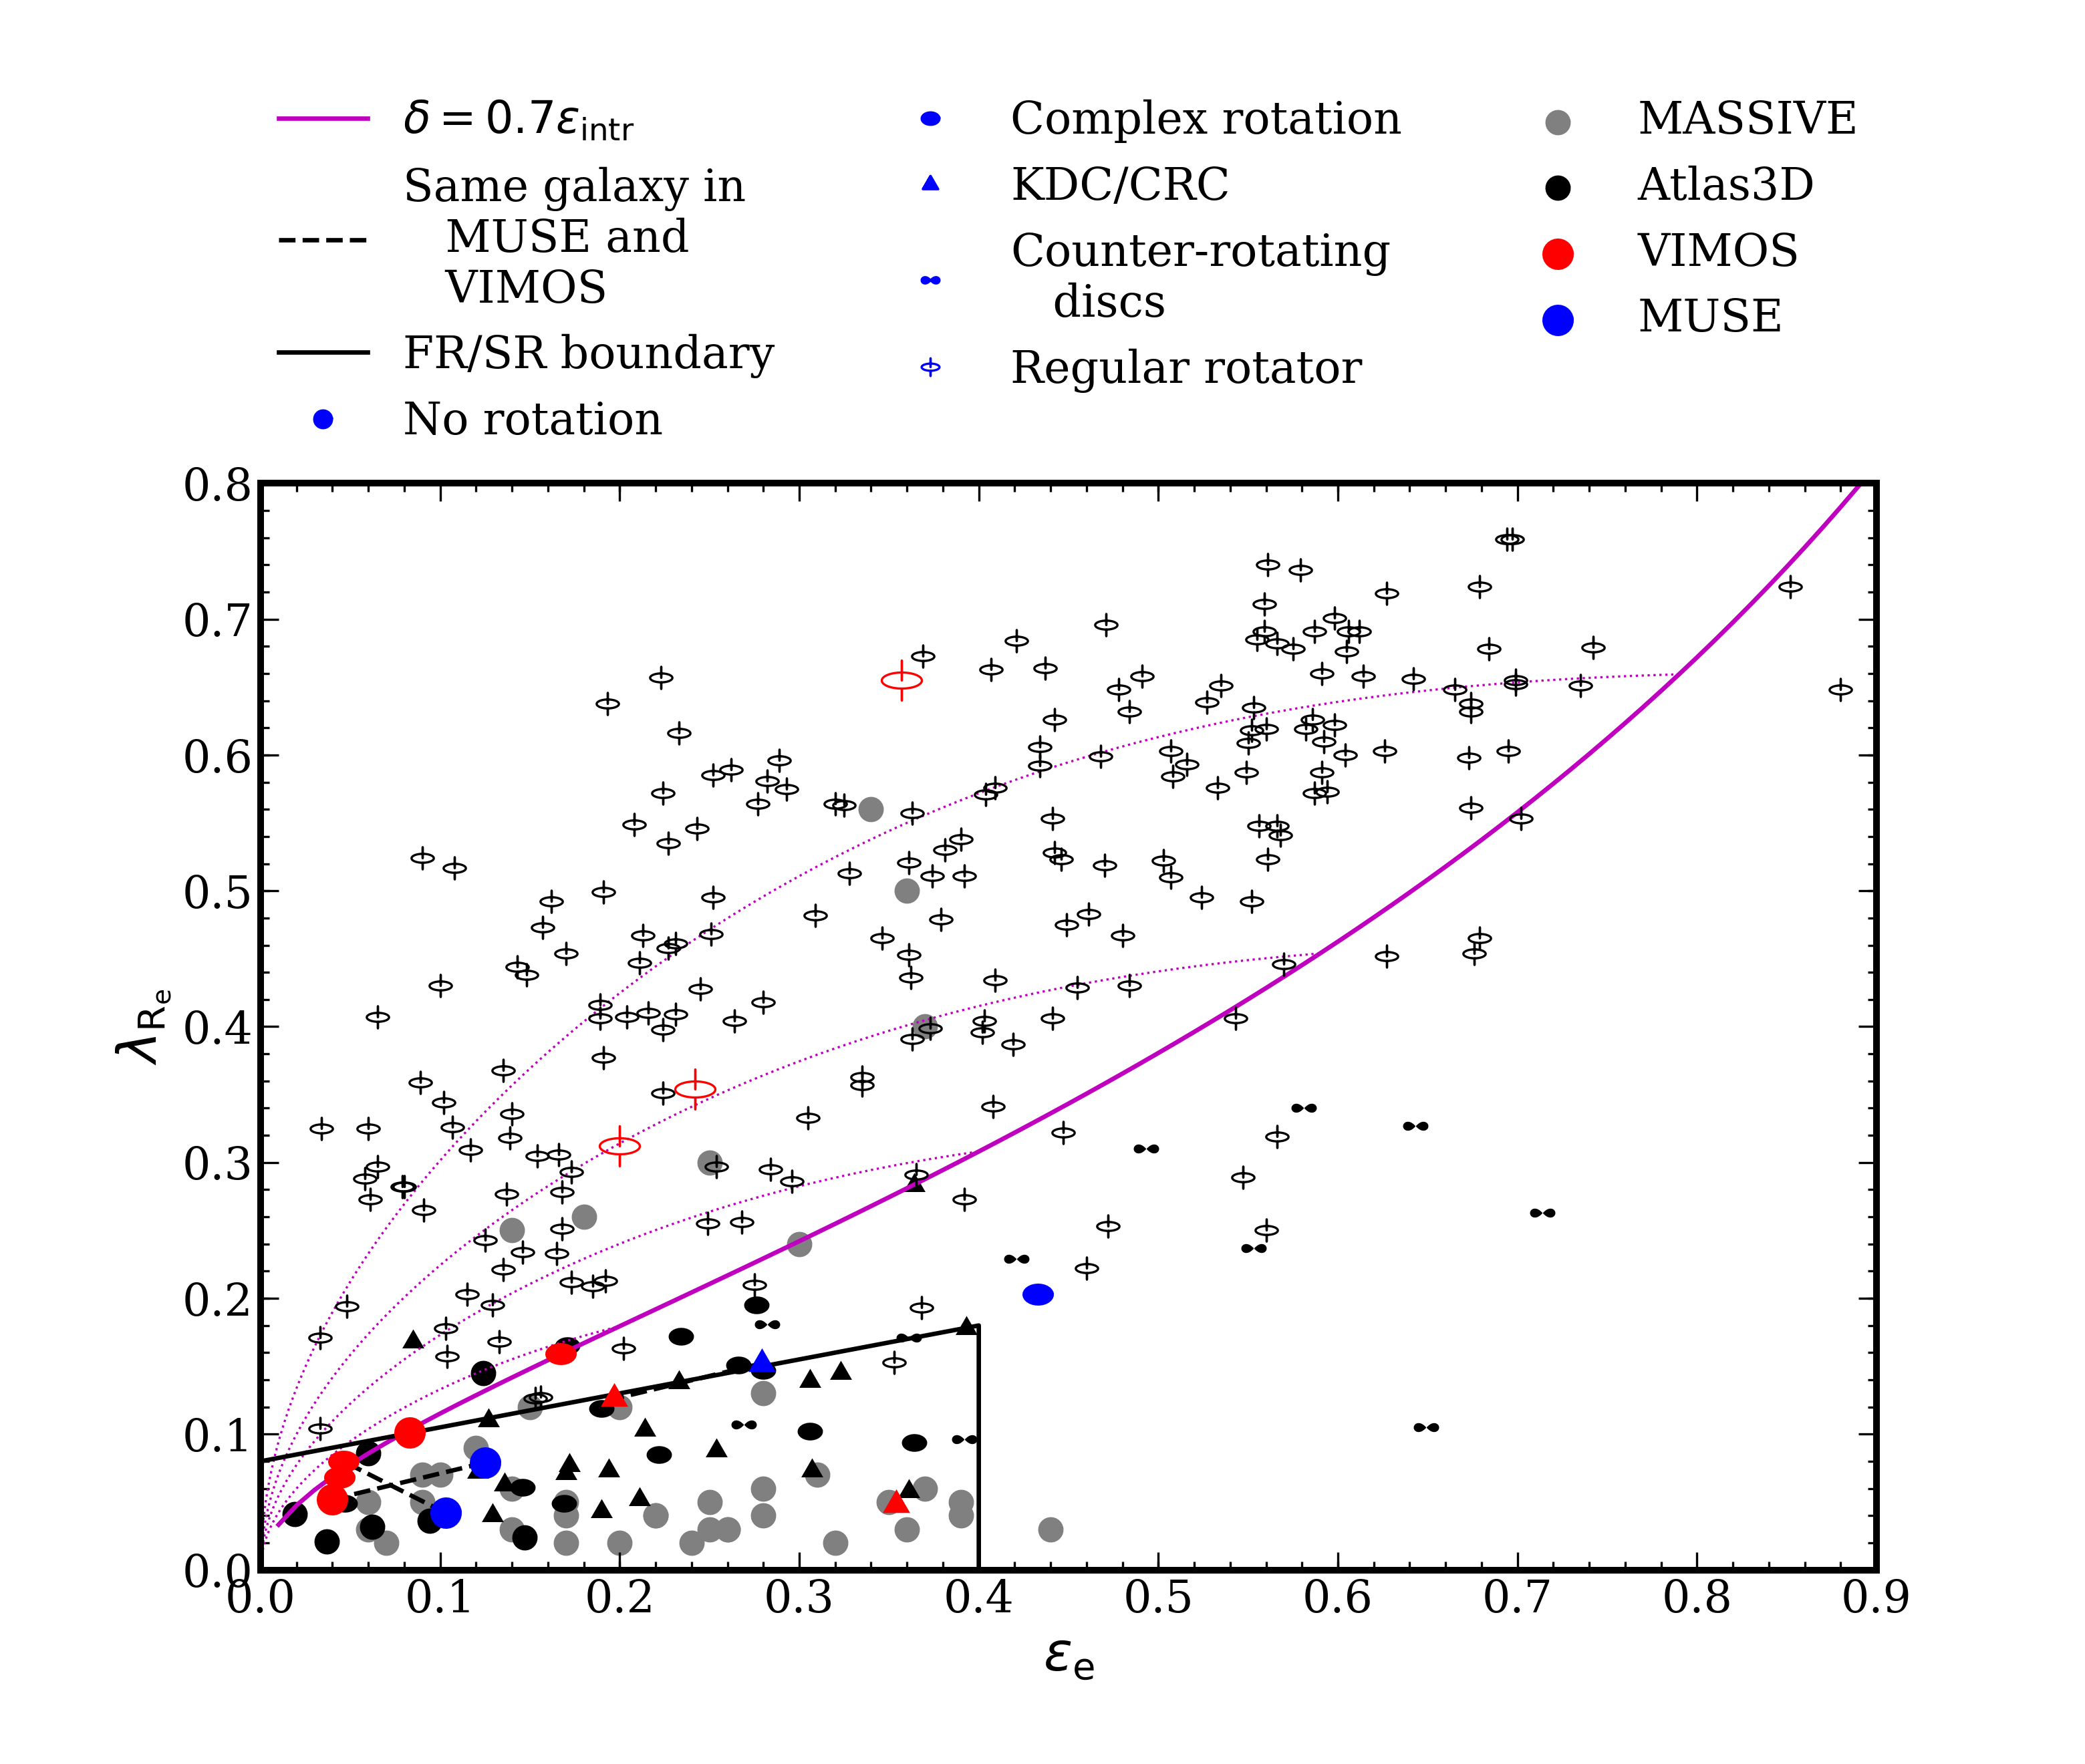
\includegraphics[width=\columnwidth]{lambda_R_ellipticity.png}
		\caption{$\lambda_\mathrm{R_e}$\,--\,ellipticity diagram. VIMOS and MUSE measurements are shown in red and blue, respectively. For comparison, Atlas$^\text{3D}$ galaxies \citep{Emsellem2011} are shown in black and MASSIVE galaxies \citep{Veale2017} in grey. The theoretical limit (edge-on systems) of disc-dominated galaxies is shown in solid magenta, with lines of constant intrinsic angular momentum but varying inclination in dotted magenta. The black solid lines show the limits of the fast-/slow-rotator classes. The MASSIVE survey does not report substructure, so the MASSIVE sample galaxies are shown with filled circles.}
		\label{fig:lambdaR_ellip}
	\end{figure}


	5 out of 11 galaxies, or $(45\pm13)$\%, are slow rotators. This is between that of the Atlas$^\text{3D}$ and MASSIVE projects, who find 13.1\% and 77.5\% of their sample galaxies to be slow rotators, respectively. As for the regular/non-regular rotators classification scheme, slow rotators are more likely to be found in higher mass galaxies and the three samples (Atlas$^\text{3D}$, MASSIVE and our Southern sample) have very different mass distributions (see upper panel of Fig.\,\ref{fig:SRmassFraction}).

	In order to account for the difference in mass distribution, we find the expected fraction of slow rotators in the Southern sample, $f'$, corrected to the mass distribution of the combined Atlas$^\text{3D}$ and MASSIVE samples (hereafter the A+M sample), as
	\begin{equation}
		f' = \sum_{i=0}^N N^\text{SS}_i f^\text{AM}_i \, , 
	\end{equation}
	where $N^\text{SS}_i$ is the number of Southern sample galaxies in the $i^\text{th}$ mass bin, $N^\text{AM}_i$ is the fraction of slow rotators in the $i^\text{th}$ mass bin in the A+M combined sample and $N$ is the total number of mass bins. In our case we use the $K$-band absolute magnitude ($M_K$) as a proxy for stellar mass, with bins of 0.5 mag. This gives an expected fraction of $f' = 0.64 \pm 0.06$, just consistent with our finding of $(45\pm13)$\% of the Southern sample galaxies being slow rotators. Again the large uncertainty reflects the low number statistics of the Southern sample. There is, therefore, no discernible difference in the fraction of galaxies that are slow-rotators between our radio-selected Southern sample and the optically-selected A+M sample, once differences in the mass distributions are taken into account. 

	\begin{figure}
		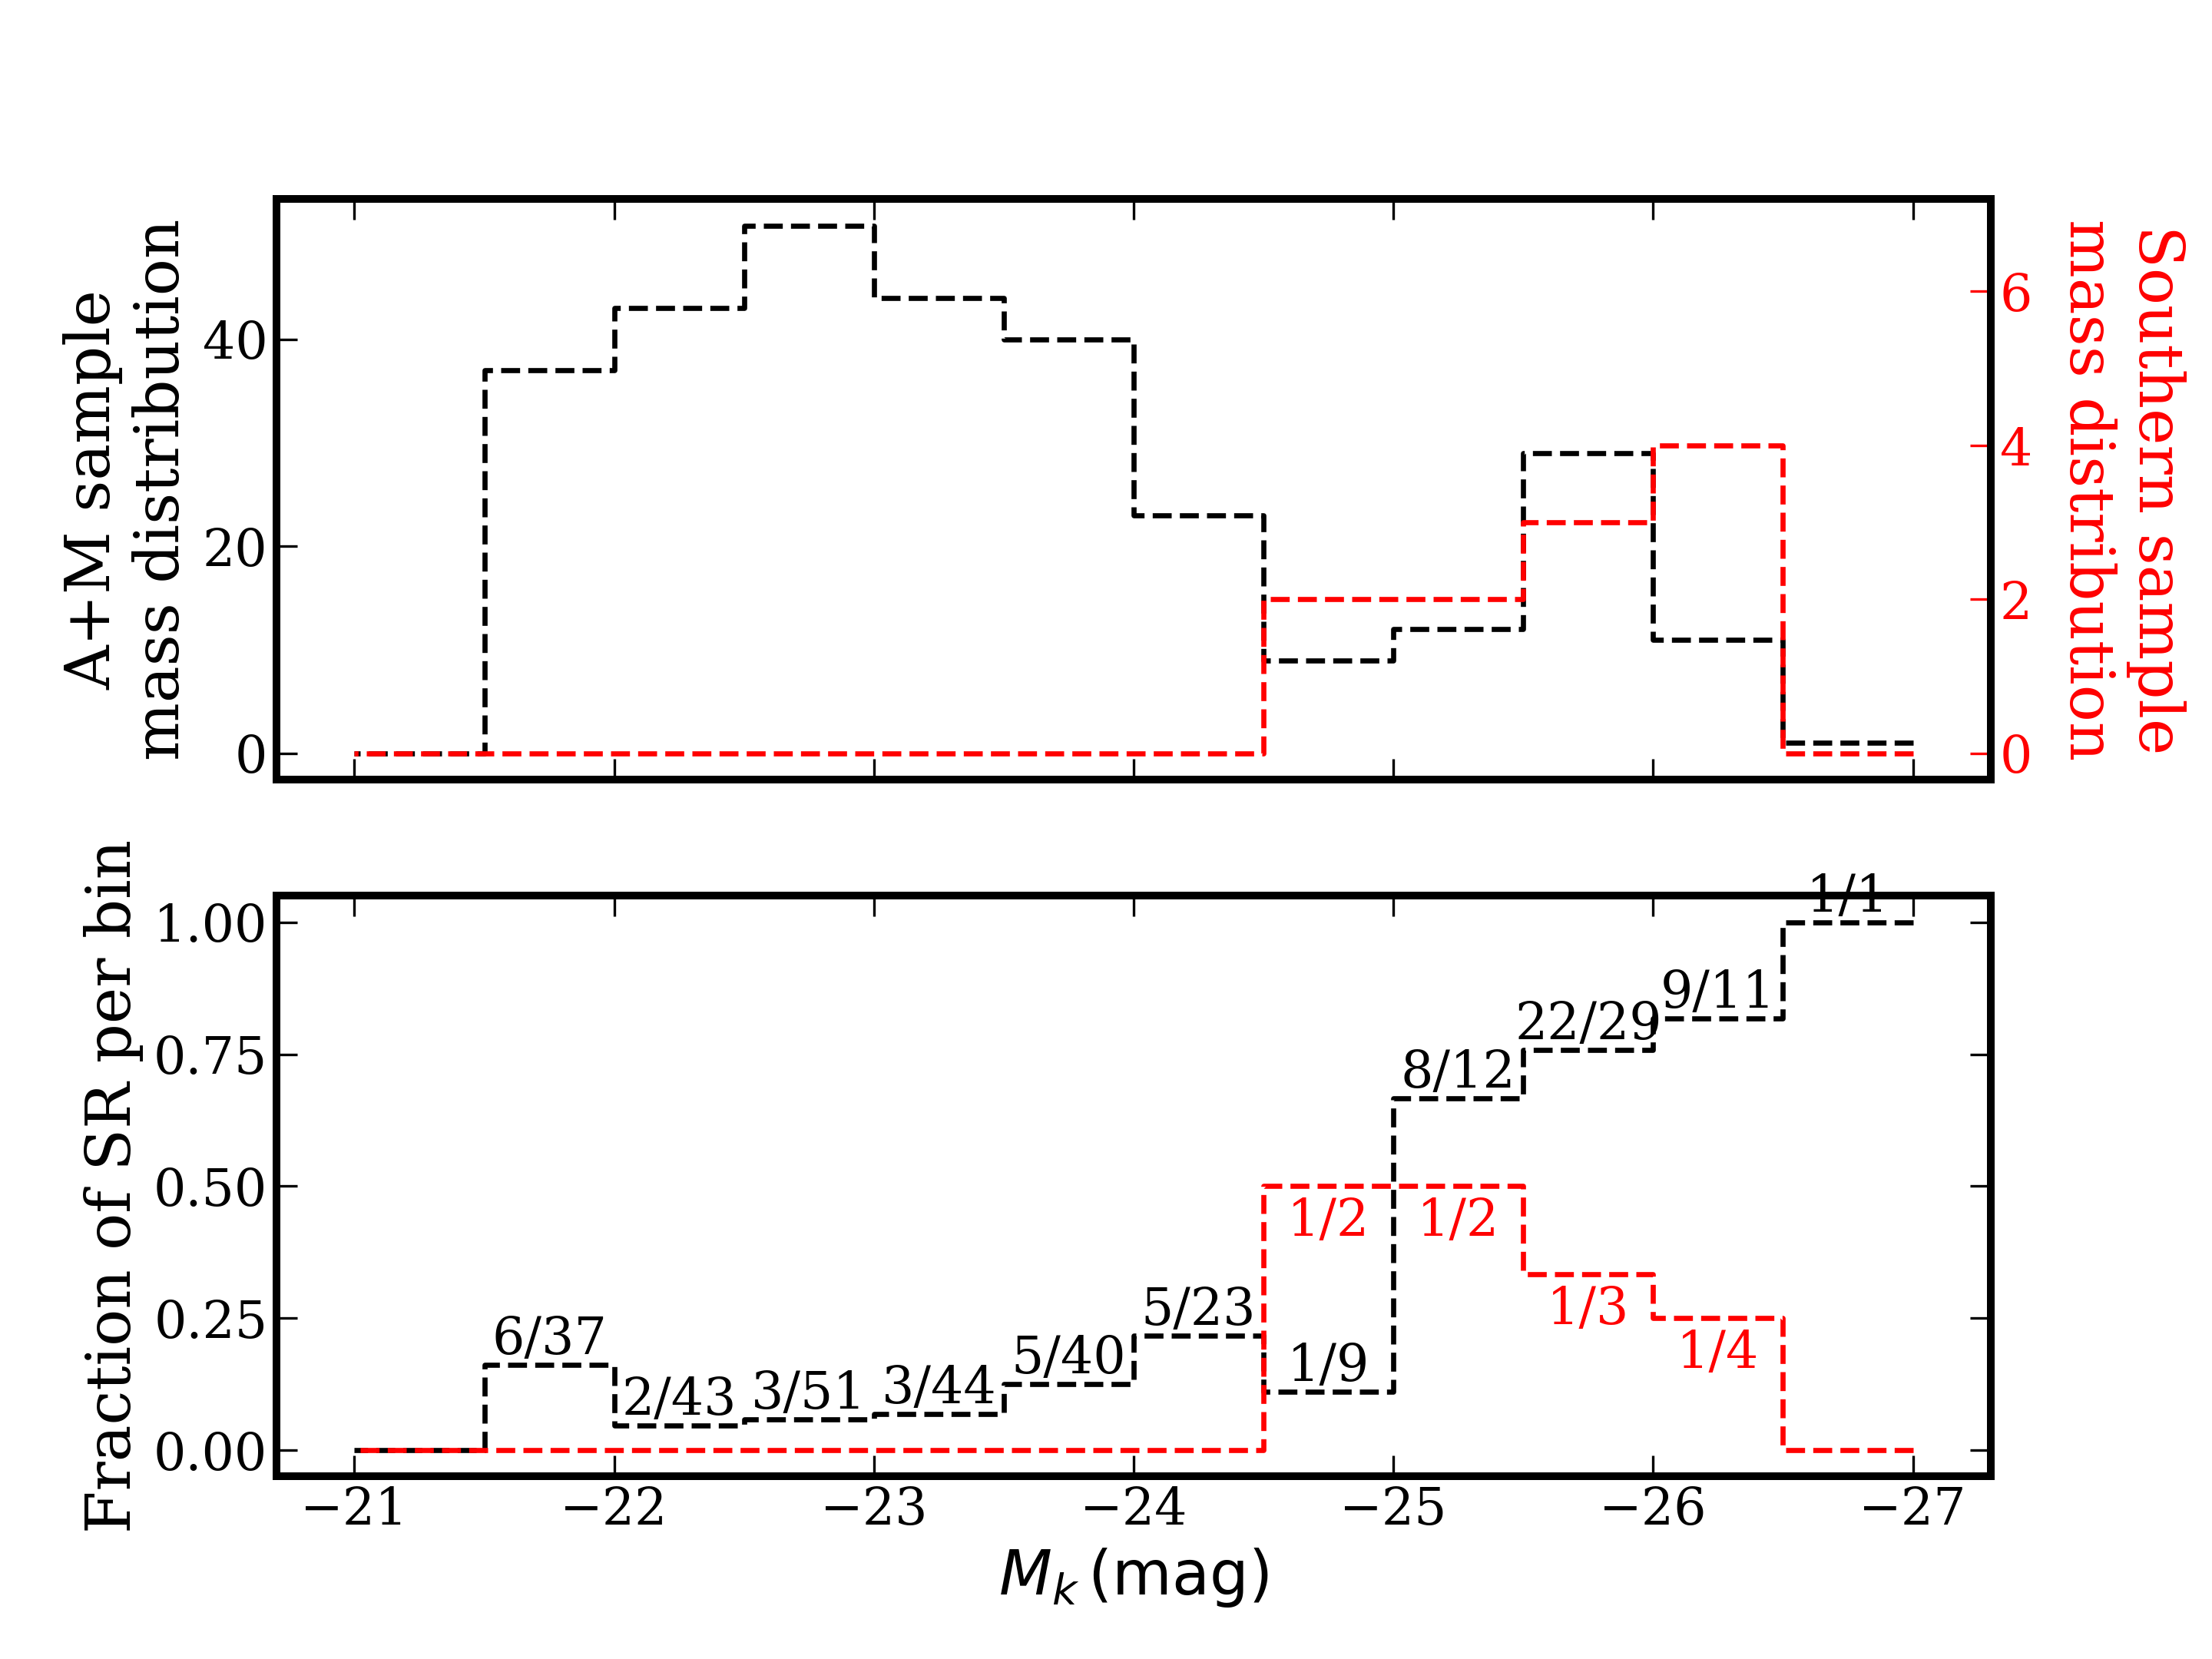
\includegraphics[width=\columnwidth]{M_k_binned.png}
		\caption{Upper panel: mass distribution of the A+M sample (black) and of our Southern sample (red). Lower panel: fraction of slow rotators within each mass bin. The labels list the number of slow rotators and total number of galaxies in each bin.}
		\label{fig:SRmassFraction}
	\end{figure}

	In addition to this, we attempt to identify the kinematic features defined by \citet{Krajnovic2011} in an algorithmic way. However, the artefacts from the VIMOS quadrants confuse ellipse fitting algorithms so only maps derived from the MUSE data are classified in this way; kinematic features in maps derived from the VIMOS data are identified by eye. These classification are listed in Col.\,7 of Table \ref{tab:classify} and the corresponding kinematic group to which a given galaxy belongs to is given is Col.\,8. We observe 3 KDCs (although PKS 718-34 is only a tentative classification) such that $29\pm19$\% of non-regular rotators in our Southern sample definitely (not including PKS 718-34) contain KDCs (or $43\pm19$\% including PKS 718-34), with the large uncertainty reflecting the low-number statistics. This is consistent with the Atlas$^\text{3D}$ survey who found find $25\pm7$\% of non-regular rotators host KDCs \citep{Krajnovic2011}.






























% Misaligned systems may appear aligned in certain projections (though aligned systems will be aligned in all projections) and as such $\Gamma_\text{kin}$ cannot be used to describe the intrinsic shape of an individual galaxy, but, as described in Section \ref{sec:ETG}, it can be used in a statistical manner. We find all the regular rotators in our Southern sample, are consistent with having aligned photometry and kinematic position angles to within 11\degree, while non-regular rotators have a large range of values of $\Gamma_\text{kin}$. IC 1531, NGC7075 and PKS 718-34 all have very large uncertainties in the value of $PA_\text{phot}$ due to the VIMOS quadrant artefacts causing the fitting routine of \textsc{kinemetry} to become unreliable. 

		% The lack of misalignments in regular rotators is consistent with \citet{Cappellari2007}, \citet{Krajnovic2011} and \citet{Fogarty2015}, who all showed that regular rotators almost always have aligned photometric and kinematic axes with very little scatter and that regular rotators with a significant misalignment are either interacting or strongly barred. The lack of misalignments suggests that the regular rotators (including those within our Southern sample) are consistent with being axisymmetric \citep{Cappellari2016}.

		% Misalignments between the photometric and kinematic position angles are routinely observed for non-regular rotators. This generally implies a more triaxial intrinsic shape, although large misalignments are extremely rarely observed in galaxies with $\epsilon > 0.4$, suggesting that non-regular rotators are more spherical in shape \citep{Cappellari2016}. The non-regular rotators in our Southern sample indeed all have $\epsilon < 0.4$ showing that they are consistent with a fairly spherical, triaxial intrinsic shape.




	

\section{Absorption Line Strengths and Stellar Populations}
	\label{sec:stellarPop}
	






\section*{Acknowledgements}

The Acknowledgements section is not numbered. Here you can thank helpful
colleagues, acknowledge funding agencies, telescopes and facilities used etc.
Try to keep it short.

%%%%%%%%%%%%%%%%%%%%%%%%%%%%%%%%%%%%%%%%%%%%%%%%%%

%%%%%%%%%%%%%%%%%%%% REFERENCES %%%%%%%%%%%%%%%%%%

% The best way to enter references is to use BibTeX:

\bibliographystyle{mnras}
\bibliography{refs} % if your bibtex file is called example.bib


%%%%%%%%%%%%%%%%%%%%%%%%%%%%%%%%%%%%%%%%%%%%%%%%%%

%%%%%%%%%%%%%%%%% APPENDICES %%%%%%%%%%%%%%%%%%%%%

\appendix
\section{Maps}
	\label{sec:Maps}

%%%%%%%%%%%%%%%%%%%%%%%%%%%%%%%%%%%%%%%%%%%%%%%%%%


% Don't change these lines
\bsp	% typesetting comment
\label{lastpage}
\end{document}

% End of mnras_template.tex